%%% Local Variables:
%%% mode: latex
%%% TeX-master: "main"
%%% End:

\chapter{Les différents modèles des taux d'interêts}

Nous avons vu dans la partie précédente que pour trouver le prix des dérivés de taux et pouvoir calculer l'espérance, il faut donner la dynamique qui régit le sous-jacent, dans notre cas  $r_t$.

Les professionnels des marchés de taux ont prix l'habitude d'évaluer les options vanille avec la formule de Black \& Scholes. Ils font l'hypothès implicite que les taux Libor $L(t, T)$ forward sont log normaux dans la mesure forward associée à leur échéance:
$$\mathrm{d} L_t(T, S) = \sigma L_t(T, S) \mathrm{d}W_t$$
Ce modèle spécifie la dynamqieu de chaque taux Libor sous sa mesure forward associées. Cependat, il est indispensable d'un point de vue pratique de pouvoir exprimer les taux Libor forward sous une même mesure. 

Diffuser des taux Libor de différentes maturitées sous une même mesure forward peut introduire des distorsions lors du traitement numéerique. En effet, les  équation montrent que plus la maturité de la mesure utilisée pour diffuser un taux Libor forward est  éloignée de $T_i$, plus le terme de tendance est important, et par conséquent plus l’erreur numérique due à une approximation pour calculer cette tendance risque d’être importante.

L'aproche historique, décrit la dynamique du taux d'interêt instantané comme étant conduite par un driver à une seule dimension. Ceci est pratique dans le sens où les prix de zéro coupon et le taux sont directement disponible dans le modèle.
De plus, certains produits financiers dépendent directement la courbe de rendement.
Nous verrons que la donnée du taux instantané $r_t$ permet de caractériser complètement courbe de taux.

Il est important que la dynamique de $r_t$ soit à la fois riche pour pouvoir décrire la courbe de rendement observée dans le marché, et suffisemment simple pour que le temps nécessaire pour le calcul ne soit trop long. Le modèle de Hull White a été introduit en 1990.
$$ \mathrm{d}r_t =  (\theta(t) - \beta(t) r_t) \mathrm{d}t + \sigma(t) \mathrm{d} W_t$$

Un des atouts majeure de ce modèle est la possiblité de simuler la dynamique de $r_t$ par un arbre. Ceci étant essentiel pour pricer des produits qui dépendent de toute une partie de la courbe de taux, et non seulement d'un point précis. Les bermuda options en sont un exemple.

\section{Le modèle à deux facteurs}
\subsection{Motivation}

Considérons un produit $E$ dont le payoff  dépent  du spread entre un taux d'intêret cumulé entre $0$ et $T_1$ pour le premier et $0$ et $T_2$ pour le second. $E$ dépend donc de la distribution jointe des deux taux.

Dans la réalité, on observe sur les marchés que les taux à différentes maturités ne sont pas corrélés. Si on regarde le taux 2Y et 10Y

\IMG{img/libor.png}{Libor}{1}


La figure suivante, tiré cours \cite{Central} reproduit une matrice de corrélation par terme de variations quotidiennes de taux zéro-coupon. Il apparait très clairement que des taux de maturités proches, comme le taux de maturité 3 ans et celui de maturité 4 ans, sont très corrélés, tandis que des taux de maturité éloignées (par exemple le taux 1 mois et le taux 10 ans) le sont très peu:

\IMG{img/tabcorr.png}{Tableau de correlation}{0.3}


\subsection{Limite des modèle à un seul facteur}
Montrons dans un premier temps pourquoi un modèle à un seul facteur n'est pas suffisant pour pricer ces produits qui dépendent non seulement de la distribution de chaque courbe de taux, mais aussi de leur corrélation. 

Rappelons la dynamique de $r_t$ dans le cadre de Hull White:
$$r_t = k(\theta - r_t)  \mathrm{d}t  + \sigma \mathrm{d}W_t$$
La formule analytique de l'obligation zéro coupon est donc
$$P(t, T) = A(t, T) exp(-B(t, T) r_t)$$
En particulier le taux d'intêret cumulé est une donné par une transformation affine du taux instantané:
$$R(t, T) = \frac{ln P(t, T)}{T-t} =: a(t, T) + b(t, T) r_t$$
Le payoff du produit $E$ est donc fonction de la distribution jointe de $R(0, T_1)$ et $R(0, T_2)$. Sauf que:
$$Cor(R(0, T_1), R(0, T_2) = 1$$

On en déduit qu'un choc à $r_t$ agit de la même manière sur toutes les courbes.


Un modèle à un seul facteur ne capture pas ce comportement. Essayons de pallier à ce problème en rajoutons un facteur à ce modèle.

Dans cette section nous considérons un modèle où le taux d'intêret instantanté est donné par une somme de deux facteurs gaussiens centrés et corrélés. Dans ce modèle doit sa popularité au fait que le prix des obligations zéron coupon admet une formule exact, ainsi que le prix des caps et des floors.


\begin{align*}
  \rm{d}x &= -\beta^y x(t) \rm{d}t + \sigma^x \rm{d}W^x_t \\
  \rm{d}y &= -\beta^y y(t) \rm{d}t + \sigma^y \rm{d}W^y_t \\
  \rm{d}r &= x + y
\end{align*}


\section{Approximation de la solution par un arbre binomial}


L'équation (*) s'intègre simplement en:
$$x(t) = x(s) e^{-\beta^y (t-s)} +  \sigma^x \int_s^t e^{- \beta^y (t-u)} \rm{d} W^x_u $$
$$y(t) = x(s) e^{-\beta^y (t-s)} +  \sigma^y \int_s^t e^{- \beta^y (t-u)} \rm{d} W^y_u $$

\subsection*{Construction}

Cette méthode a été d'abord suggéré par Hull-White (1994)

On discrétise l’intervalle $[0, T]$ avec les temps $T_i = i \Delta t$, où $\Delta t = \frac{T}{N}$.
Nous donnons une approximation de la dynamique processus $x$ et $y$, par une suite de variable de discretisé $((\widetilde{x}_i, \widetilde{y}_i) \approx (x(i \Delta i), (y(i \Delta t))_i $. Pour celà nous calculerons les deux premier moment de $(x, y)$.

Nous faisons le calcul pour $x$, la même formule s'appliquera à $y$.
$$E(x(t+\Delta t) | F_t) = x(t) e^{-a \Delta t}$$
$$V(x(t+\Delta t) | F_t) = \frac{{\sigma^x}^2}{2a} (1 - e^{-2a \Delta t})$$
$$Cov\{x(t+\Delta t), y(t+\Delta t) | F_t \} = \frac{\sigma^x \sigma^y \rho}{a + b} (1-e^{-(a+b)\Delta t})$$

Pour que le $((\widetilde{x}_i, \widetilde{y}_i)$ et $(x(i \Delta i), (y(i \Delta t))_i $ aient les même moment, la loi de  $((\widetilde{x}_i, \widetilde{y}_i)$  est donnée par:
$$\mathrm{P} \left( \widetilde{x}_{i+1} = \widetilde{x}_i + a \, \mathrm{d}x, \widetilde{y}_{i+1} = \widetilde{y}_i + b \, \mathrm{d}y |  \widetilde{x}_i, \widetilde{y}_i \right) = p^{a, b}( \widetilde{x}_i, \widetilde{y}_i)$$
où 
\begin{itemize}
\item $a, b \in \{-1, +1\}$
\item $p$ est donnée par:
$$ p^{a, b}(x, y) = \frac{1 + a \rho}{4} - b \frac{\beta^y \sigma^x y + a \sigma^x \sigma^y  x}{4 \sigma^x \sigma^y} \sqrt{\Delta t} $$
\end{itemize}

Le schéma suivant résume les transitions du processus {$(\widetilde{x}, \widetilde{y})$};
%%% Local Variables:
%%% mode: latex
%%% TeX-master: "main.tex"
%%% End:

\tikzstyle{bag} = [text width=10em, text centered]
\tikzstyle{end} = []
\begin{figure}[h!]
  \centering
\begin{tikzpicture}[sloped]
  \node (xy) at (0,0) [bag] {$(\widetilde{x}, \widetilde{y})$};
  \node (a) at ( 3,-2) [bag] {$(\widetilde{x} + \rm{d}x, \widetilde{y} + \rm{d}y)$};
  \node (b) at ( -3,-2) [bag] {$(\widetilde{x} + \rm{d}x, \widetilde{y} - \rm{d}y)$};
  \node (c) at ( 3,2) [bag]{$(\widetilde{x} - \rm{d}x, \widetilde{y} + \rm{d}y)$};
  \node (d) at ( -3,2) [bag]{$(\widetilde{x} - \rm{d}x, \widetilde{y} - \rm{d}y)$};
  \draw [->] (xy) to node [below] {$p^{+, +}$} (a);
  \draw [->] (xy) to node [below] {$p^{+, -}$} (b);
  \draw [->] (xy) to node [above] {$P^{-, +}$} (c);
  \draw [->] (xy) to node [above] {$p^{-, -}$} (d);
\end{tikzpicture}
\end{figure}






Nous appelons slice l'ensemble des noeuds qui sont équi distant de la racine. Une slice représente la distribution du processus $( \widetilde{x}_i, \widetilde{y}_i)$ à un instant donné.

Le pricing se fait en deux temps:
\begin{itemize}
\item On diffuse le processus $(\widetilde{x}, \widetilde{y})$ dans l'arbre en prenant soin de calculer la probabilité de transition d'un état à un autre
\item On ``drawback'' dans l'arbre en partant de la date à laquelle on fait le payoff, en ***discountant***
\end{itemize}

  \subsection*{Petite discussion sur la courbe d'actualisation vs la courbe de diffusion}
  Avant la crise de 2008, il était d'usage courant que les banques considèrent le taux Libor comme reflétant la réalité du marché de crédit inter-bancaire. Le taux est publié quotidiennement par
taux réél auquel les banques sont prête à se prétter de l'argent est appelé taux OIS (Overnight Index Swap).  
Pendant la crise, le spread entre LIBOR et OIS était si grand qu'il devenait impossible à ignorer. Depuis tous les modèles de taux intégrent deux courbe, une pour la diffusion (LIBOR par exemple) et une autre pour l'actualisation (OIS).
Dans le développement de cet article, nous ignorons cette différence.
  
\section{Améliorations}
Si nous implémentons l'abre de façon naîve (voir \ref{fig:oldtree} ), le nombre de noeuds augmente de façon exponentielle en fonction du nombre de pas de temps. En pratique ceci est problématique et conduit vite à une saturation de mémoire. Dans l'exemple simplifié ci-dessus nous traçons l'arbre de diffusion du premier facteur ($x(t)$). A chaque pas de temps le nombre de noeuds double, ie pour $n$ pas de temps, nous nous retrouvons avec $2^n$ noeuds pour un facteur, ou $4^n$ pour deux. 

%%% Local Variables:
%%% mode: latex
%%% TeX-master: t
%%% End:

% Define styles for bags and leafs
\tikzstyle{bag} = [text width=2em, text centered]
\tikzstyle{end} = []
\begin{figure}[H]
  \centering
\begin{tikzpicture}[sloped]
  \node (a) at ( 0,0) [bag] {$0$};
  \node (b) at ( 4,-1.5) [bag] {$- \sigma \Delta t$};
  \node (c) at ( 4,1.5) [bag] {$+ \sigma \Delta t$};
  \node (d) at ( 8,-3) [bag] {$-2 \sigma \Delta t$};
  \node (e1) at ( 8,0.5) [bag] {$+ 0 \sigma \Delta t$};
  \node (e2) at ( 8,-0.5) [bag] {$+ 0 \sigma \Delta t$};
  \node (f) at ( 8,3) [bag] {$+ 2 \sigma \Delta t$};
  
  \draw [->] (a) to node [below] {$p^-$} (b);
  \draw [->] (a) to node [above] {$p^+$} (c);
  \draw [->] (c) to node [below] {$p^+$} (f);
  \draw [->] (c) to node [above] {$p^-$} (e1);
  \draw [->] (b) to node [below] {$p^+$} (e2);
  \draw [->] (b) to node [above] {$p^-$} (d);
\end{tikzpicture}
\caption{Arbre construit de façon naïve}
\label{oldtree}
\end{figure}



Remarquer que $(x, y)_i$tilde est un processus markovien homogène à valeurs discrètes nous permet d'optimiser la simulation de l'arbre. En effet, il nous suffit de calculer la table de transition une fois au début du programme et de la réutiliser pour avancer/reculer dans le temps. (voir \ref{fig:newtree})


%%% Local Variables:
%%% mode: latex
%%% TeX-master: t
%%% End:

% Define styles for bags and leafs
\tikzstyle{bag} = [text width=2em, text centered]
\tikzstyle{end} = []
\begin{figure}[H]
  \centering
  \begin{tikzpicture}[sloped]
  \node (a) at ( 0,0) [bag] {$0$};
  \node (b) at ( 4,-1.5) [bag] {$- \sigma \Delta t$};
  \node (c) at ( 4,1.5) [bag] {$+ \sigma \Delta t$};
  \node (d) at ( 8,-3) [bag] {$-2 \sigma \Delta t$};
  \node (e) at ( 8,0) [bag] {$+ 0 \sigma \Delta t$};
  \node (f) at ( 8,3) [bag] {$+ 2 \sigma \Delta t$};
  \draw [->] (a) to node [below] {$p^-$} (b);
  \draw [->] (a) to node [above] {$p^+$} (c);
  \draw [->] (c) to node [below] {$p^+$} (f);
  \draw [->] (c) to node [above] {$p^-$} (e);
  \draw [->] (b) to node [below] {$p^+$} (e);
  \draw [->] (b) to node [above] {$p^-$} (d);
\end{tikzpicture}
\caption{Arbre optimisé}
\label{newtree}
\end{figure}




Voir l'annexe pour l'implémentation en python.
Ci-dessous une visualisation graphique de plusieurs slices à différents instants, nous rappelons qu'une slice est l'ensemble des valeurs possibles d'une fonction aléatoire, le prix d'une obligation zéro coupon en loccurence, à un instant précis.

\begin{figure}[H]
 \begin{minipage}[b]{.46\linewidth}
  \centering    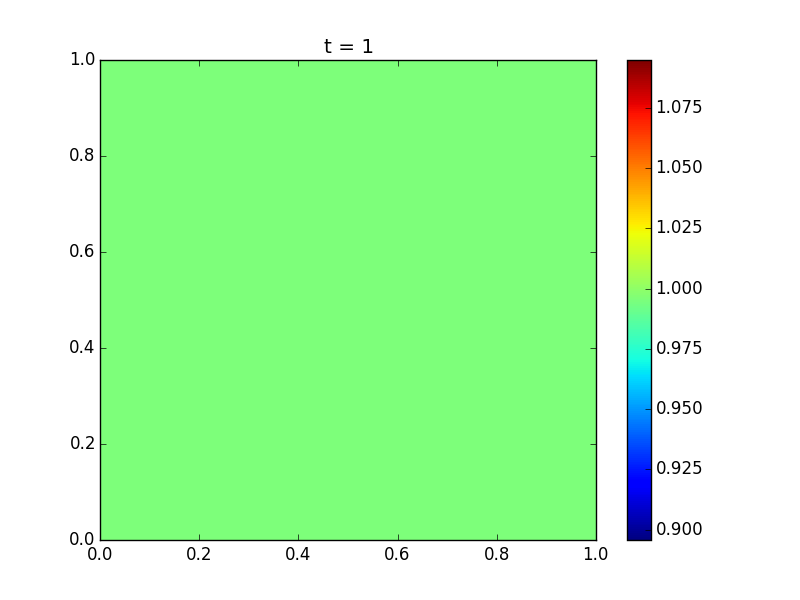
\includegraphics[scale=0.2]{img/slices2d/sl_1.png}
  \caption{$t = 1$ \label{fig1}}
 \end{minipage} \hfill
 \begin{minipage}[b]{.46\linewidth}
     \centering    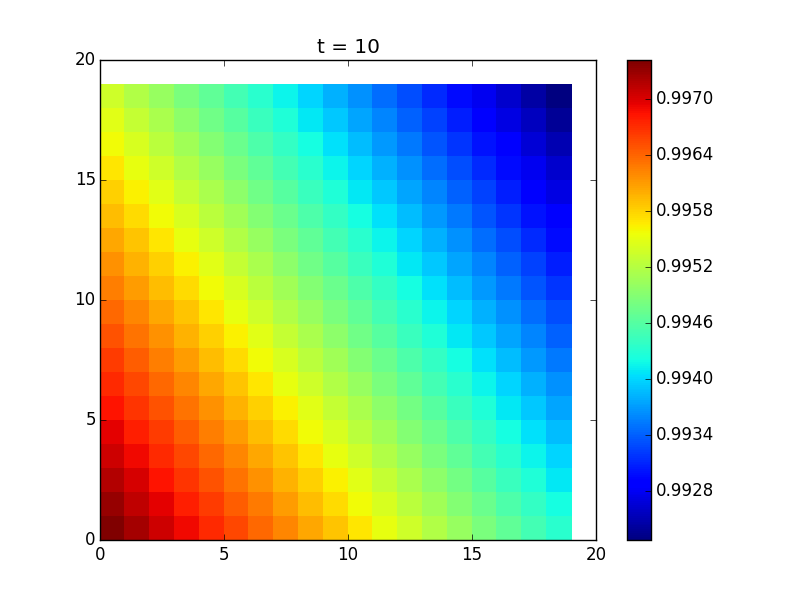
\includegraphics[scale=0.2]{img/slices2d/sl_10.png}
  \caption{$t = 10$ \label{fig2}}
\end{minipage}
 \begin{minipage}[b]{.46\linewidth}
     \centering    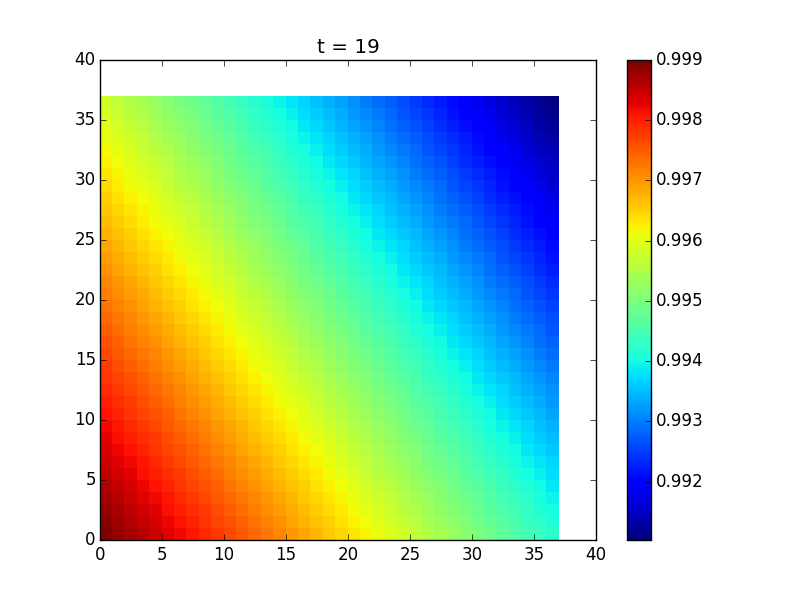
\includegraphics[scale=0.2]{img/slices2d/sl_19.png}
  \caption{$t = 20$ \label{fig3}}
\end{minipage}
 \begin{minipage}[b]{.46\linewidth}
     \centering    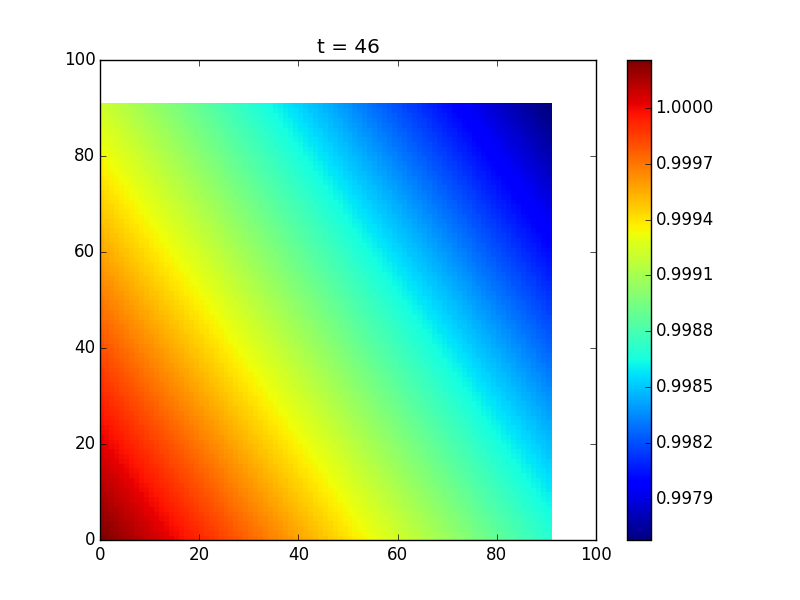
\includegraphics[scale=0.2]{img/slices2d/sl_46.png}
  \caption{$t = 30$}
\end{minipage}

\end{figure}

Une autre améliroation possible est de trouver une formule analytique pour certain produits. En effet, si nous reprenons l'exemple d'un cancellable spread option 2Y10Y dont la maturité est dans 5 ans, nous devrions normalement construite l'arbre jusqu'en 2030 pour avoir le taux 10Y en 2020. Nous pouvons éviter celà en fournissant directement une formule exacte pour les zéro coupons. C'est ce que nous faisons dans la partie suivante.

\subsection{Formule exacte}
Cette partie est fortement insipiré de \cite{Brugo}.

On rappelle l'expression du prix de l'obligation zéron coupon sous la mesure risque neutre $Q$
$$P(t, T) = \espr{ e^{-\int_t^T r_u \rm{d}u}} $$

Notons $I(t, T) := \int_t^T x(u) + y(u) \rm{d}u$, et montrons que conditionnellement à l'information accumulé jusqu'au temps $t$, que c'est une variable normale d'espérance $M(t, T)$ et de variance $V(t, T)$ où:
\begin{align}
  M(\beta^y, t, T) &:= \frac{1 - e^{-\beta^y (T-t) }}{\beta^y} \\
  V(\beta^y, \sigma^x, \beta^y, \sigma^y, t, T) &:= \frac{\sigma^x \sigma^y}{\beta^y \beta^y} \left[ T - t + \frac{e^{-\beta^y (T-t) } - 1}{\beta^y} + \frac{e^{-\beta^y (T-t) } - 1}{\beta^y} - \frac{e^{-(\beta^y + \beta^y) (T-t) } - 1}{\beta^y + \beta^y} \right] \\
  V(t, T) &:= V(\beta^y, \sigma^x, \beta^y, \sigma^x, t, T)
            + V(\beta^y, \sigma^y, \beta^y, \sigma^y, t, T)
            + 2 \rho V(\beta^y, \sigma^x, \beta^y, \sigma^y, t, T) \\
            M(t, T) &:= M(\beta^y, t, T) x(t) + M(\beta^y, t, T) y(t)
\end{align}

\begin{proof}
  Par simple calcul \cite{Brugo}:
  $$  \int_t^T x(u) \rm{d}u = \frac{1 - e^{-\beta^y (T-t)}}{\beta^y} + \frac{\sigma^x}{\beta^y} \int_t^T \left[1 - e^{-\beta^y (T-t)}\right] \rm{d} W^x_u$$
  $$  \espr{\int_t^T x(u) \rm{d}u} = M(\beta^y, t, T) x(t)$$
  $$ Var(\int_t^T x(u) \rm{d}u) =   \left(\frac{\sigma^x}{\beta^y}\right)^2 \espr{ \int_t^T \left[1 - e^{-\beta^y (T-t)}\right]^2 \rm{d}u } = V(\beta^y, \sigma^x, \beta^y, \sigma^x, t, T)$$ (isométrie d'itto)
\end{proof}

Nous avons donc
\begin{align}
  P(t, T) &= exp  \left(  -\int_t^T r_u \rm{d}u + \frac{1}{2} Var \left( {-\int_t^T r_u \rm{d}u} \right)  \right) \\
          &= exp  \left( - M(\beta^y, t, T) x(t) - M(\beta^y, t, T) y(t) + \frac{1}{2} V(t, T) \right)
  \end{align}

Nous utiliserons cette formule directement dans le pricer, ce qui nous évitera de construire l'arbre jusqu'à la date de maturité du dernier zéro coupon.

Pour mesurer l'impact de ce changement sur le temps d'execution du programme, nous avons utilisé le logiciel \textbf{valegrind}. Ce logiciel  permet le profilage du code, ie il permet de controler:
\begin{itemize}
\item la liste des fonctions appelées et le temps passé dans chacune d'elles
\item l'utilisation processepur
\item l'utilisation mémoire
\end{itemize}

Ci-dessous deux graphes produits par le logiciel qui illustre le nombre de fois que la fonction responsable de l'évolution de l'arbre \mintinline{cpp}{Hyb4_UpdateStatePricesOnly} est appelée:

\IMG{img/ycso2.png}{En utilisant l'arbre pour le calcul des $P(t, T)$}{0.5}
\IMG{img/ycso3.png}{En utilisant la formule exacte}{0.5}

Le nombre d'appels à cette fonction est environ réduit de moitié. Cette dernière étant très gourmande en ressource, le temps total requis par le programme est réduit de $~30\%$.

\subsection{Ajout d'un shift déterministe}
Le modèle, tel que développé jusqu'a présent, présente un inconvénient majeur: à tout instant, $r_t$ est symétriquement distribué autour de $0$. Ceci ne correspond pas à la réalité, puisque les taux négatifs ne sont observé dans les marchés que dans de très rares circonstance ( en Europe après crise inter-bancaire de 2009, Au Japon après des années de déflation ). Une autre raison est que le modèle ne permet pas de retrouver les prix des obligations zéro coupon.

Pour pallier à ce problème, nous rajoutons une fonction $\phi$ au taux $r_t$. La fonction déterministe $\phi(t)$ permet de fitter exactement la courbe de taux observée. Dans la partie ``Calibraion nous'' nous verrons comment calculer cette fonction à partir des prix de bonds zéro coupon.

En prenant en compte ce changement, le prix de l'obligation zéro coupon devient:

$$P(t, T) = \espr{ e^{-r_t + \phi(t)}}$$

Nous prendrons soin de modifier l'étape de ``draw back'' dans l'abre en changeant le facteur d'actualisation.

Le processus est markovien

\subsection{Optimiser la taille des slices }

La slice que nous avons construite est rectangulaire.
La plage que nous autorisons à $(x, y)$ doit logiquement dépendre de leur corrélation. Ainsi pour simuler deux processus parfaitement corrélés, il suffit de simuler l'un deux, la slice dans ce cas est simplement linéaire. Dans le cas ou ils sont indépendants, il est nécessaire de simuler les deux, et la slice sera parfaitement rectangulaire. Dans le cas général nous utilisons la méthode suivante 

Nous décomposons la source de stochasticité $dW_t$ en deux composantes indépendantes:
$$ \rm{d} W_t := (\rm{d} W^x_t, \rm{d} W^y_t)^T = A(t)  \rm{d}Z_t$$
où
$$
A(t) := 
\left(
  \begin{array}{cc}
            \sigma^x & 0  \\
            \rho \sigma^y & \sqrt{1-\rho^2} \sigma^y \  \\
  \end{array}
\right)
$$
$Z = (Z^1, Z^2)$ un mouvement brownien 2D à compostantes indépendantes.

A l'instant $t_n$,
$$x(t_{n+1}) := x_i(t_n) (1 - \beta^y \Delta) + ... Z_1$$
$$y(t_{n+1}) := y_i(t_n) (1 - \beta^y \Delta) + ... Z_1 + ...Z_2$$
Les limites de l'abre sont définie comme étant les bords de l'ellipsoid décrit par l'équation:

$$Z_1^2 + Z_2^2 \leq n_{\sigma^x}^2$$

Où $n_{\sigma^x}$ est sans unité et dénote le dégré de déviation de la moyenne qu'on autorise.


\subsection{ Paramètres dépendant du temps}

Dans la partie précédente, les paramètres ($\sigma^x, \sigma^y, \beta^y, \beta^y, \rho)$ étaient constantes. Pour plus de souplesse, nous considérons des variables qui dépendent  du temps, ou plus précisément constantes par morceaux.

Le calcul du prix des obligtions zéro coupon est fourni en annexe.

Deux problèmes cependant avec cette méthode:

\begin{itemize}
\item Le calcul est beaucoup plus long
\item possibilité de overfitter les données historique du marché, ce qui affecte négativement le pouvoir prédicitive du modèle
\end{itemize}


